\documentclass{article}
\usepackage{graphicx}
\usepackage{amssymb}
\usepackage{amsmath}
\usepackage{float}
\usepackage{hyperref}
\usepackage[margin=1in]{geometry}

\begin{document}

\title{Robotics 811 - HW 3 - Resubmit}
\author{Xiang Zhi Tan}
\maketitle

\section{Q1}
\subsection*{1(c)}
This question was done with help and discussion from Reuben Aronson\\
As we are trying to approximate the function with a quadratic functions($n = 2$), by the theorem given in the class and notes, we know there are $n+2$ points that are $\varepsilon ||f-p||_\infty$, which are the maximum error of the best quadratic approximation function. Our approximation function could be written in the following form
\begin{equation*}
p(x) = a + bx + cx^2
\end{equation*}
However, a quick observation of the graphing of the function(as seen in question 1(b)), we can see that the function $f(x)$ is actually an odd function, shown by how the values of $f(x), where\;x<0$ is just the reflection of $f(x),where\;x>0$ along the $y = -x$ line. As a odd functions will be best approximate by another odd functions, that simplifies our approximation function to:
\begin{equation} \label{eq:2}
p(x) = bx
\end{equation}
From the theorem, we know that the error function $E(x) = \|f-p\|_{\infty}$ is maximized at 4 points, that allows us to construct the following equations
\begin{equation*}
\begin{aligned}
e(x_0) &= f(x_0) - p(x_0) = sinh(x_0) - b(x_0)\\
e(x_1) &= f(x_1) - p(x_1) = sinh(x_1) - b(x_1)\\
e(x_2) &= f(x_2) - p(x_2) = sinh(x_2) - b(x_2)\\
e(x_3) &= f(x_3) - p(x_3) = sinh(x_3) - b(x_3)
\end{aligned}
\end{equation*}
By the theorem, as $f^{n+1}(x)$ does not change sign on [a,b], we know that $x_0 = -2$ and $x_1 = 2$. We also know that as a maximum error point, the first derivative of the error function at that point must be $0$. The derivative of $e(x)$ is as following, and we can represent the function in terms of x
\begin{equation} \label{eq:1}
\begin{aligned}
e'(x) = cosh(x) - b =& 0\\
cosh(x) = & b\\
x = \pm cosh^{-1}(b)
\end{aligned}
\end{equation}  
Because all the errors are the same values with different signs, we now that $e(x_2) = - e(x_3)$. By substituting equation \ref{eq:1} into that equation, we will get following equation
\begin{equation*}
sinh(cosh^{-1}(b)) - b(cosh^-1(b)) = - sinh(2) + 2b
\end{equation*}
By solving the previous equation numerically, we get
\begin{equation*}
b \approx 1.600233
\end{equation*}
This will give us our approximation function by substituting b into equation \ref{eq:2}.
\begin{equation*}
p(x) = 1.600233x
\end{equation*}
\begin{figure}[H]
\centering
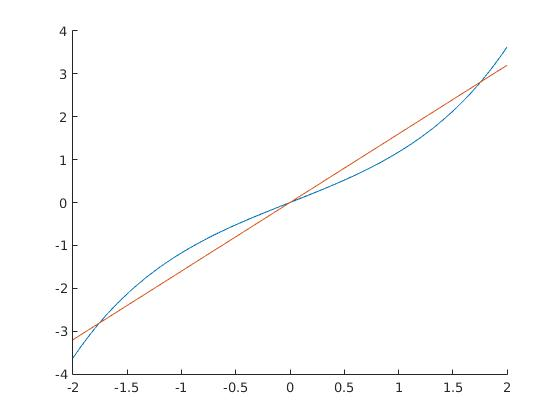
\includegraphics[width=5in]{figures/q1c.jpg}
\caption{graph of $f(x) = sinh(x)$ over [-2 2] with the approximation function, $p(x) = 1.600233x$}
\end{figure}
Now we will determine the $L_\infty$ and $L_2$ error of the approximation function. $L_\infty$ error would be the just the error function used in the approximation.
\begin{equation*}
\begin{aligned}
|e(x_0)| &= sinh(-2) - 1.600233(-2)\\
	&\approx 0.4264
\end{aligned}
\end{equation*}
$L_2$ error can be found through integration of the error function
\begin{equation*}
\begin{aligned}
\int_{-2}^2(f(x) - p(x))^2 &= \sqrt{\int_{-2}^2(sinh(x) - bx)^2}\\
							&\approx \sqrt{0.354438}\\
							&\approx 0.595347
\end{aligned}
\end{equation*}

\subsection*{1(d)}
Now we will be approximating the best least squares approximation by a quadratic function. First we will construction a orthogonal sequence of polynomials with the given interval using the recurrence function given in page 33 of the notes on approximation. We will define $p_0(x) \equiv 1$. Following is the construction of $p_1(x)$ and $p_2(x)$.
\begin{equation}\label{eq:3}
\begin{aligned}
&<p_0,p_0> &= \int_{-2}^2 1 dx = 4\\
&<xp_0,p_0> &= \int_{-2}^2 x dx = 0\\
p_1(x) &= [x - 0]p_0(x) = x\\
&<p_1,p_1> &= \int_{-2}^{2} x\cdot x dx = \frac{16}{3}\\
&<xp_1,p_1> &= \int_{-2}^{2} x^2\cdot x dx = 0\\
p_2(x) &= [x - 0]p_1(x) - \frac{\frac{16}{3}}{4} = x^2 - \frac{4}{3}\\
&<p_2,p_2> &= \int_{-2}^{2} (x^2 - \frac{4}{3}) \cdot (x^2 - \frac{4}{3}) dx = \frac{256}{45}\\
\end{aligned}
\end{equation}
Now we want to project the function $f(x)$ on the subspace spanned by the polynomials(basis) that we generated. Which can be done with the following formula:
\begin{equation*}
p(x) = \sum_{i=0}^{2} \frac{<f(x),p_i>}{<p_i,p_i>}p_i(x)
\end{equation*}
Where $p_i$ are the polynomial we generated in equation \ref{eq:3}. Here we will calculate $<f(x),p_i>$ for all $i$.
\begin{equation*}
\begin{aligned}
<f(x),p_0> = \int_{-2}^2 sinh(2) \cdot 1 dx &= cosh(x)|_{-2}^2 \\
& = 0\\
<f(x),p_1> = \int_{-2}^2 sinh(2) \cdot x dx &= x cosh(x)|_{-2}^2 - sinh(x)|_{-2}^2 \\
& = 7.7951\\
<f(x),p_2> = \int_{-2}^2 sinh(2) \cdot (x^2 - \frac{4}{3}) dx &= (x^2 - \frac{4}{3}) cosh(x)|_{-2}^2 -2(x sinh(x)|_{-2}^2 - cosh(x)|_{-2}^2)\\
& = 0\\
\end{aligned}
\end{equation*}
Let $d_i$ be $\frac{<f(x),p_i>}{<p_i,p_i>}$. Then,
\begin{equation*}
\begin{aligned}
d_0 &= \frac{0}{4} = 0\\
d_1 &= \frac{7.7951}{\frac{163}{3}} \approx 1.4616\\
d_2 &= \frac{0}{\frac{256}{45}} = 0
\end{aligned}
\end{equation*}
These will give us our least square approximation of
\begin{equation} \label{eq:4}
p(x) = 1.46146p_i(x) = 1.4616x
\end{equation}
\begin{figure}[H]
\centering
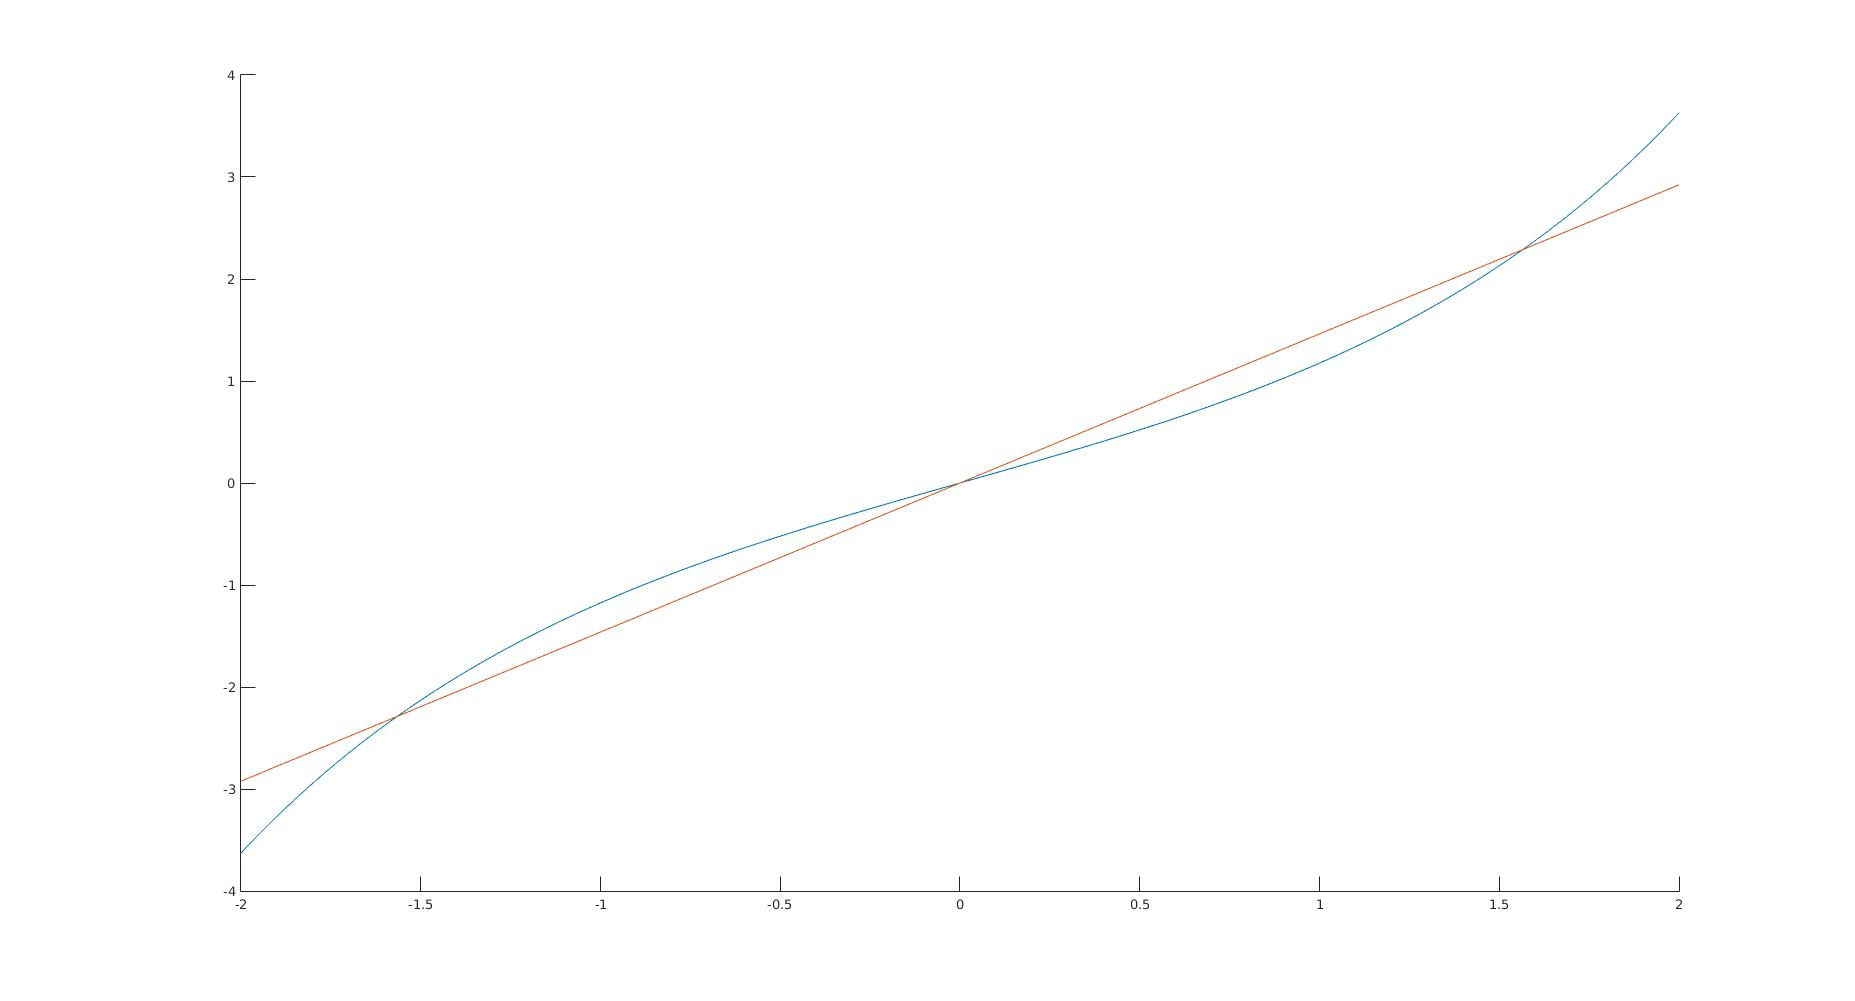
\includegraphics[width=5in]{figures/q1d.jpg}
\caption{graph of $f(x) = sinh(x)$ over [-2 2] with the approximation function $p(x) = 1.4616x$}
\end{figure}
Now we will determine the $L_\infty$ and $L_2$ error of the approximation function. The $x$ value that will give the $L_\infty$ error would either be the at the boundaries or when the derivative of the error function is $0$.
\begin{equation*}
\begin{aligned}
e(x) = (f(x) - p(x))^2 &= (sinh(x) - 1.4616x)^2\\
e'(x) &= 2(sinh(x) - 1.4616x)(cosh(x) - 1.4616) = 0\\
x &\approx \pm 0.927255\\
x &= 0 \\
x &\approx \pm 1.56559\\
\end{aligned}
\end{equation*}
This means $x$ for the maximum error would be either $2$,$-2$ or one of the x in the previous equation. After substituting all x in equation \ref{eq:4}. We found the maximum error given from all x is $0.7037$ at the points $x = 2$ and $x = -2$.\\
$L_2$ error can be found through integration of the error function
\begin{equation*}
\begin{aligned}
\int_{-2}^2(f(x) - p(x))^2 &= \sqrt{\int_{-2}^2(sinh(x) - 1.4616x)^2}\\
							&\approx \sqrt{0.251898}\\
							&\approx 0.501894
\end{aligned}
\end{equation*}

\section{Q4}
The solution of this question was based on a similar problem on a computer vision homework that was done this semester.
\subsection*{4(a)}
We are trying to solve the plane equation $ax +by + cz = d$, where $<a,b,c>$ will be the normal vector of the plan. Because we are using the least square methods, that means we are trying find best parameters, $v$ which are $<a,b,c,d>$ such that $Av = 0$, where $A$ are the input variables. This is equal to try minimize $|Av|^2$ subjecting to the fact that $|v| = 1$ such that it is a non trivial solution.\\
We do the minimization of $|Av|^2$ through SVD as the minimum of the equation is equal to the eigenvector of A corresponding to the smallest eigenvalue. We decompose $A$ into $[U \Sigma V]$ where $\Sigma$ is the eigenvalues of $A$. We pick the smallest eigenvalue and the corresponding eigenvector in $V$. The eigenvector will be least square solution to our plane equation.\\
The implementation of this algorithm is done in the file \textbf{planeSolver.m} where the function will return the least square $[a,b,c,d]$ solution given a set of input points. The least square approximation of the plane equation is:
\begin{equation*}
-0.0853x - 0.8920y - 0.0436z = 0.4418
\end{equation*}
Following is the figure of the approximated plane from 2 different angles. The code to generate the graph can be found in \textbf{q4a.m}
\begin{figure}[H]
\centering
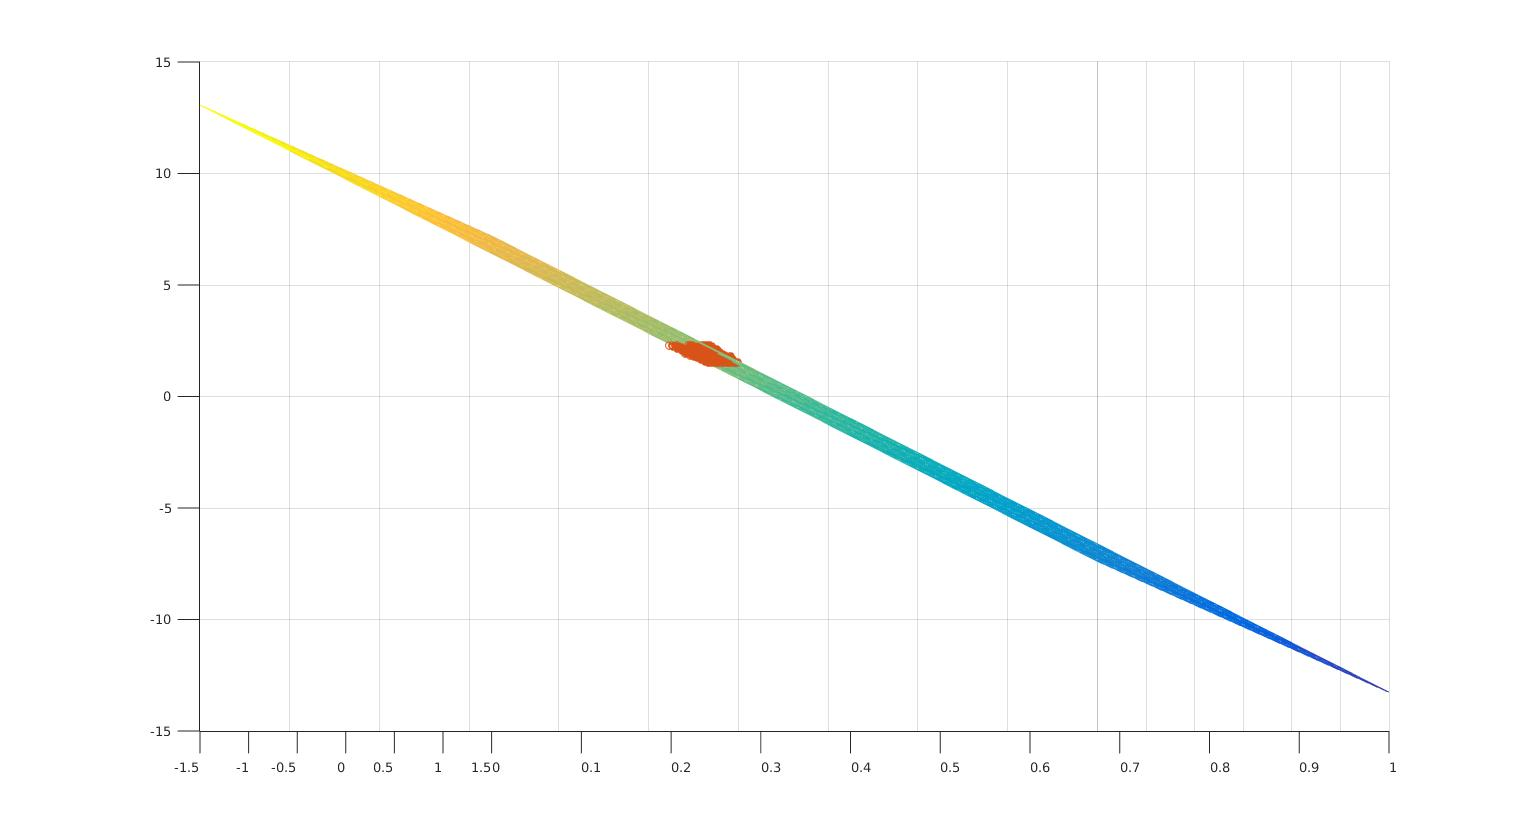
\includegraphics[width=5in]{figures/q4a_1.jpg}
\end{figure}
\begin{figure}[H]
\centering
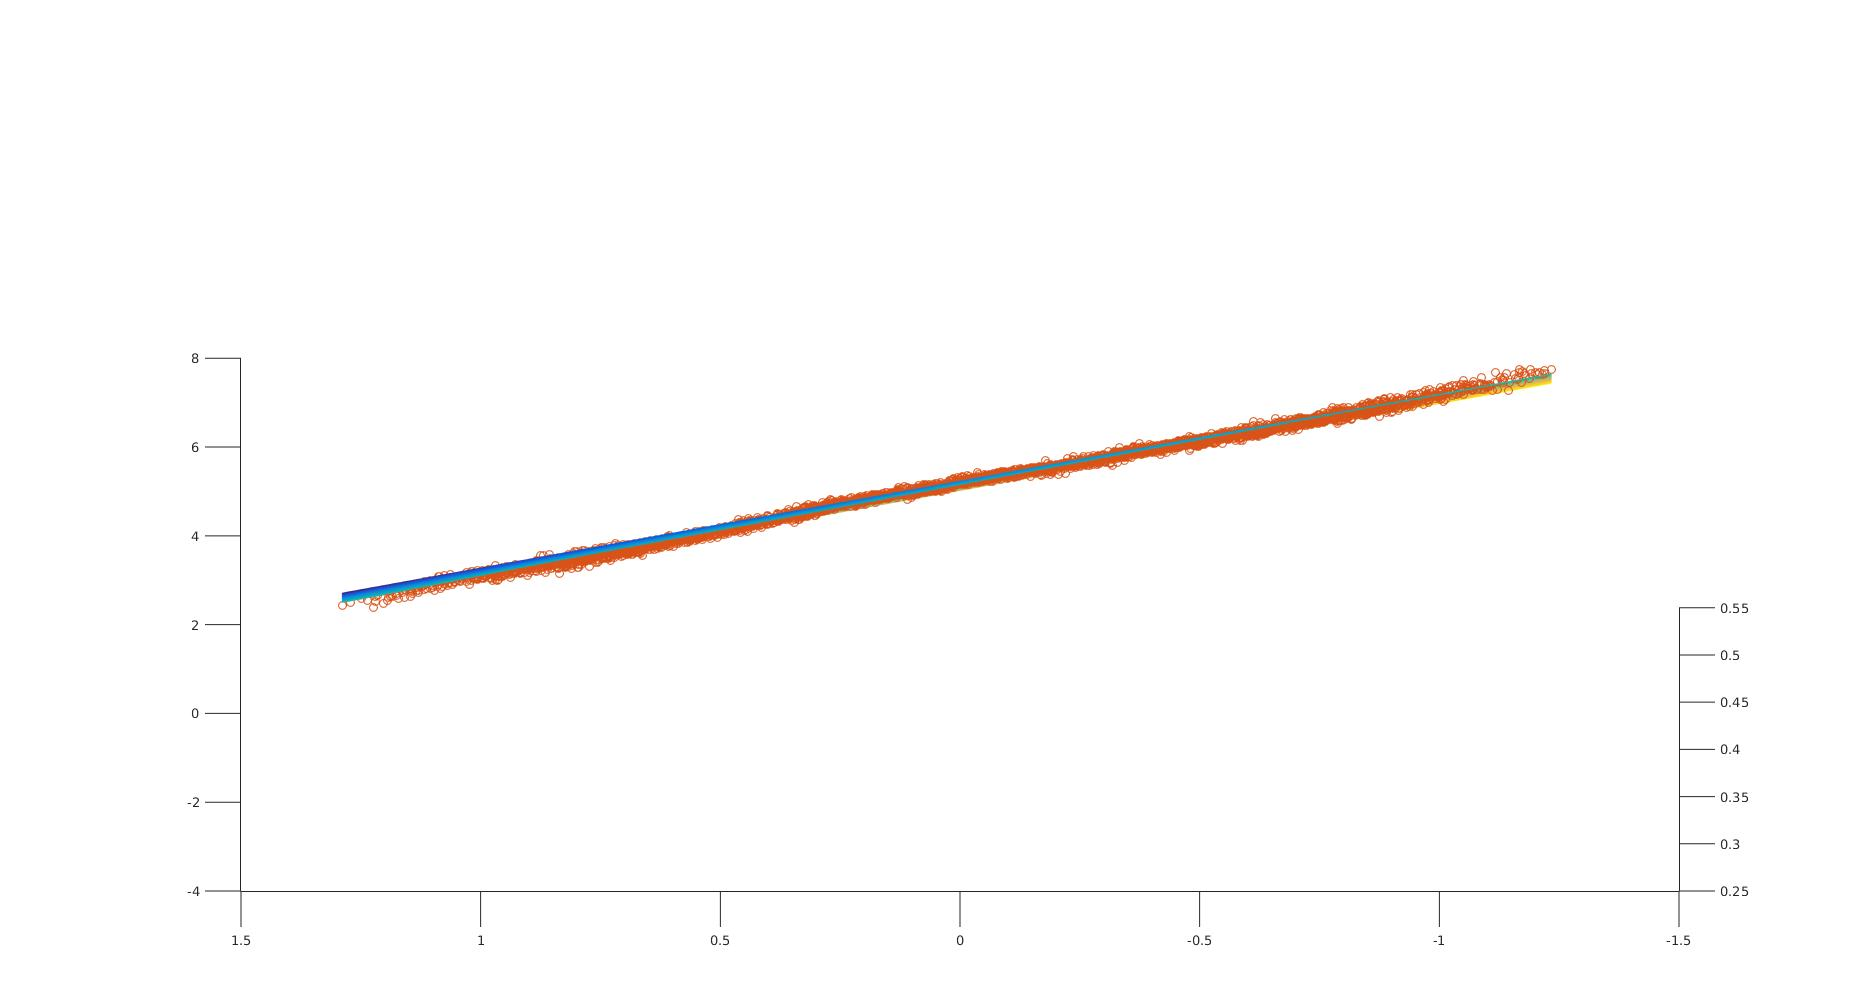
\includegraphics[width=5in]{figures/q4a_1-alt.jpg}
\end{figure}
The average distance from the plane to each point is $0.0027$, which is pretty good.

\subsection*{4(b)}
Using the same method, we see that the plane is no longer aligned to the points and have an average distance to each point of $0.0248$ which is 10 times the error of a.
\begin{figure}[H]
\centering
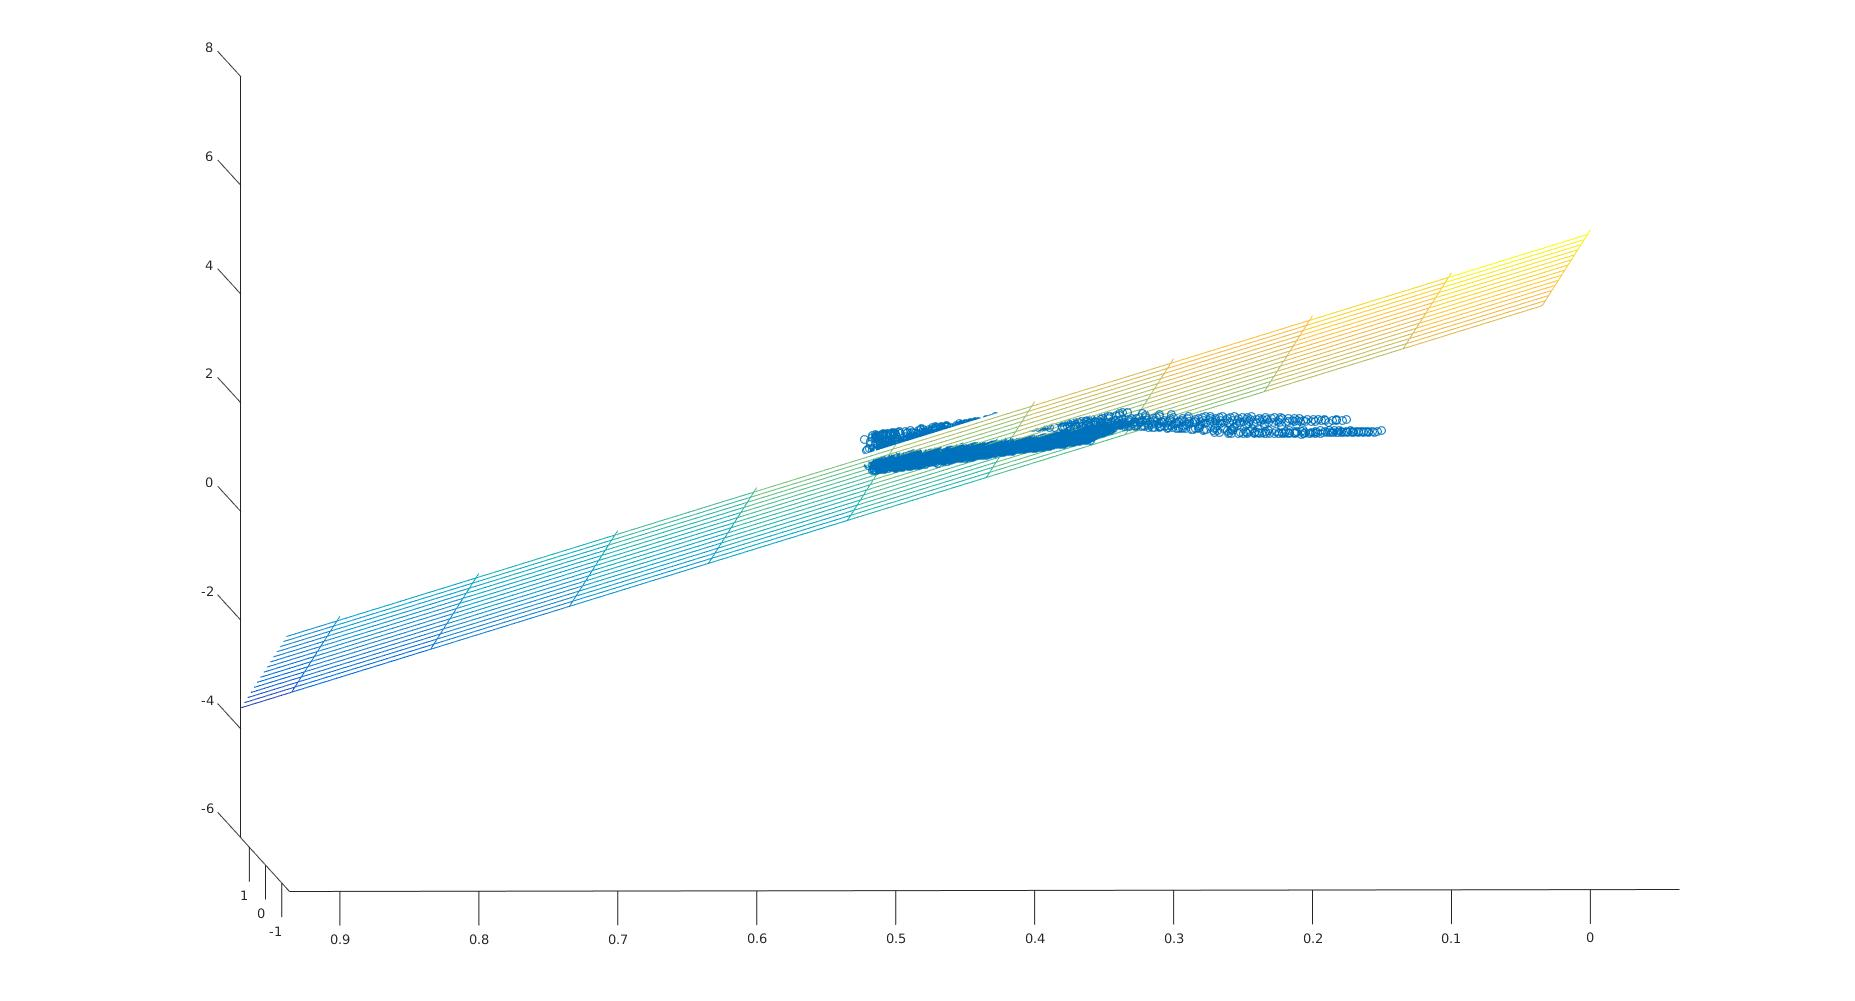
\includegraphics[width=5in]{figures/q4b.jpg}
\caption{note how the plane does not follow the plane points}
\end{figure}

\subsection*{4(c)}
To solve this issue, we choose to use the RANSAC algorithm to filter out outlier points. Our implementation of RANSAC does the following it.\\
First, it picks 4 random points. Using, these 4 points, we create a plane equation. we then measure the average distance of each point to the plane. If the point has a distance less than the \textbf{tolerance}, the points are consider as \textbf{inliers}. we loop through this process for \textbf{n iterations}, and save all the \textbf{inliers} for the iteration with the highest \textbf{inliers} count. After n iterations, we generate a new plane equation with the \textbf{inliers}. The implementation of RANSAC can be found in \textbf{RANSAC.m}.\\
Using this method, we found $3015$ inliers from the $3537$ given points. The average distance from the inliers to the plane was $0.002$ Following is the figures of the approximated plane from 2 different angles. The code to generate the graph can be found in \textbf{q4c.m}
\begin{figure}[H]
\centering
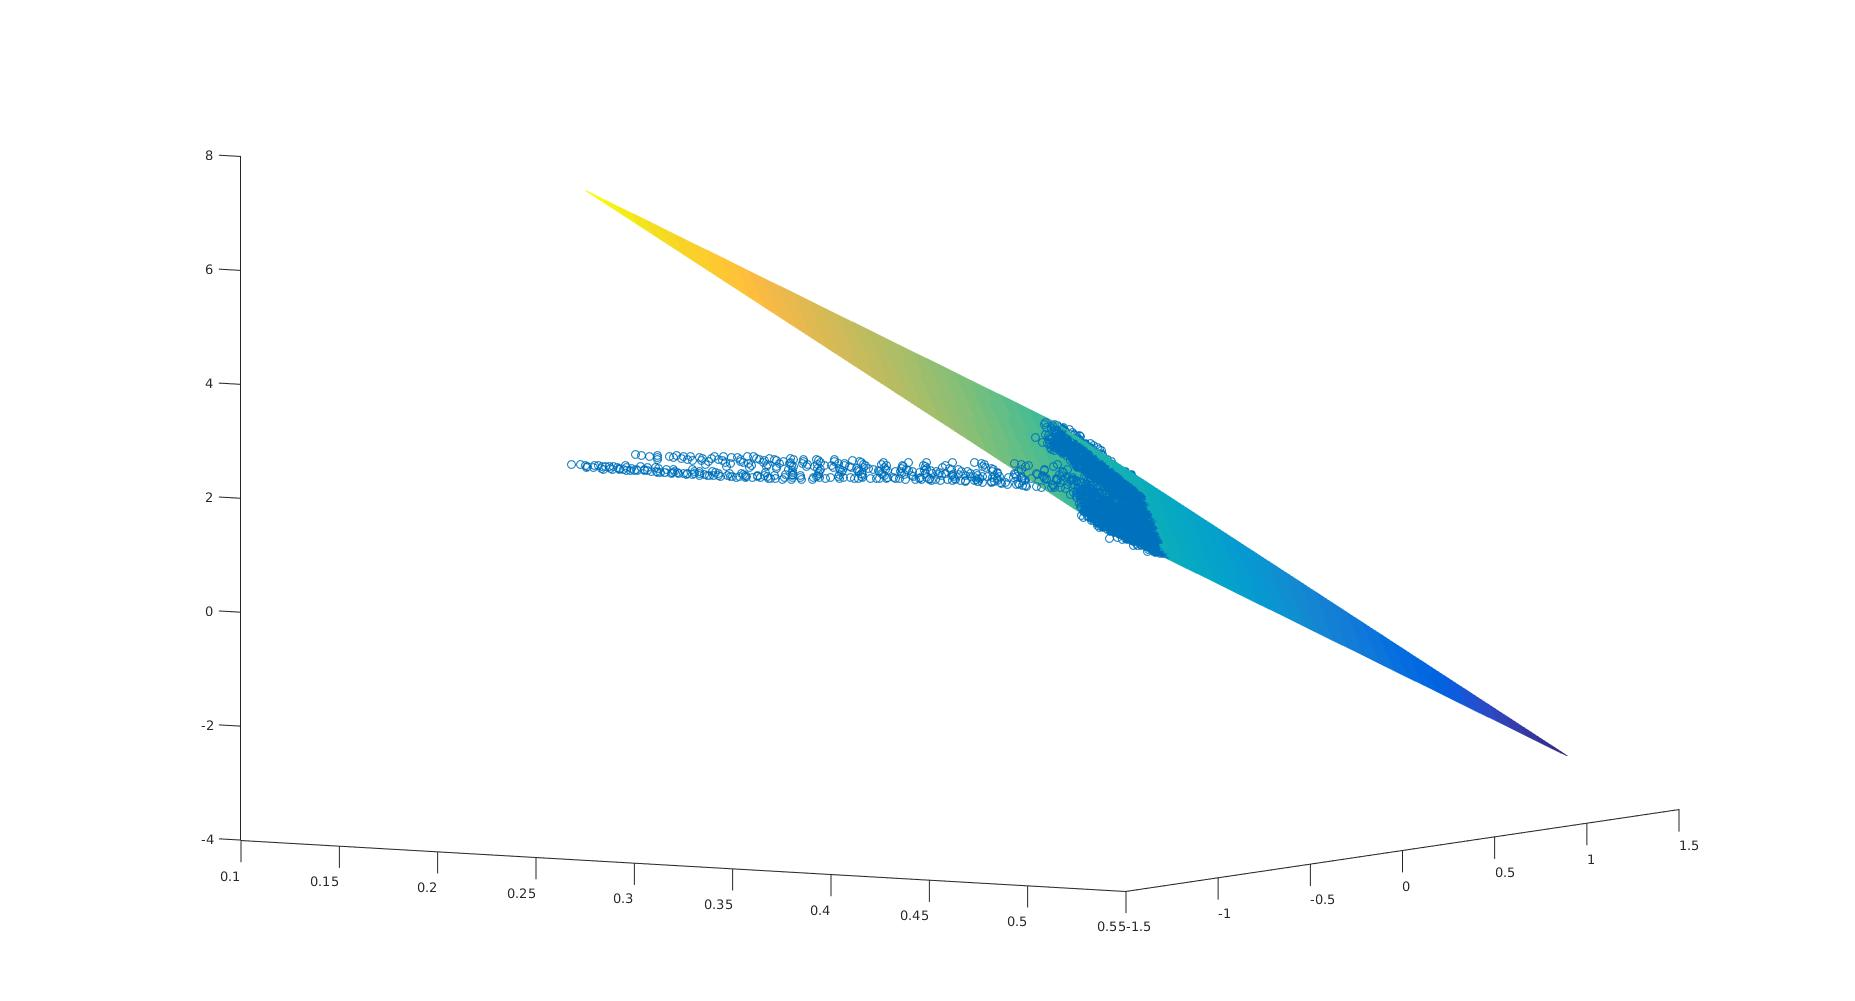
\includegraphics[width=5in]{figures/q4c.jpg}
\end{figure}
\begin{figure}[H]
\centering
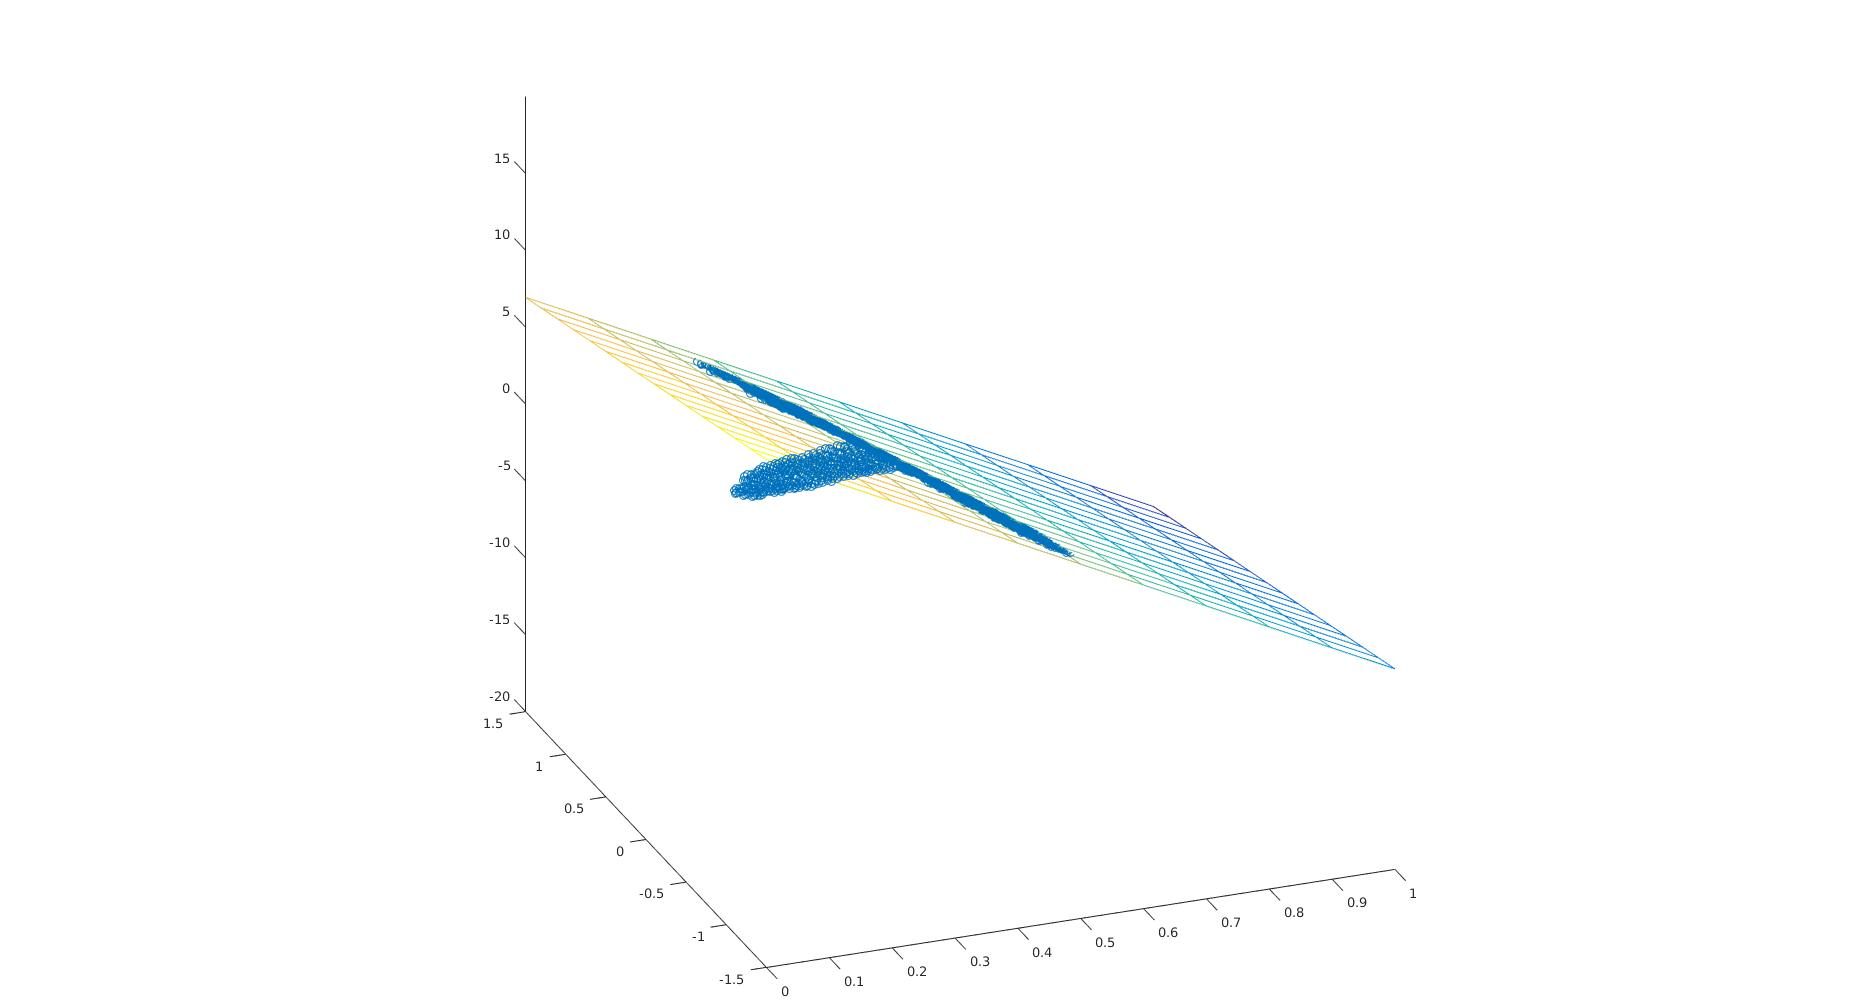
\includegraphics[width=5in]{figures/q4c-alt.jpg}
\end{figure}

\subsection*{4(d)}
The improved RANSAC will now ran the RANSAC algorithm 4 times(not iterations, but the whole alogirthm). First, It will find a plane equations that have the maximum possible number of points, then It will remove those points from the list and run RANSAC algorithm on the remain points. After 4 iterations, by theory, the algorithm should end up with 4 different plane equations that have the maximum number of inliers. The code for this improved RANSAC can be found in \textbf{RANSAC\_improved.m}.\\
Using the improved algorithm, we found 4 planes with $3090,2720,2060$ and $1291$ points respectively. Following is the visualization of the data and 4 planes from 2 different angles. The code to generate the graph can be found in \textbf{q4d.m}
\begin{figure}[H]
\centering
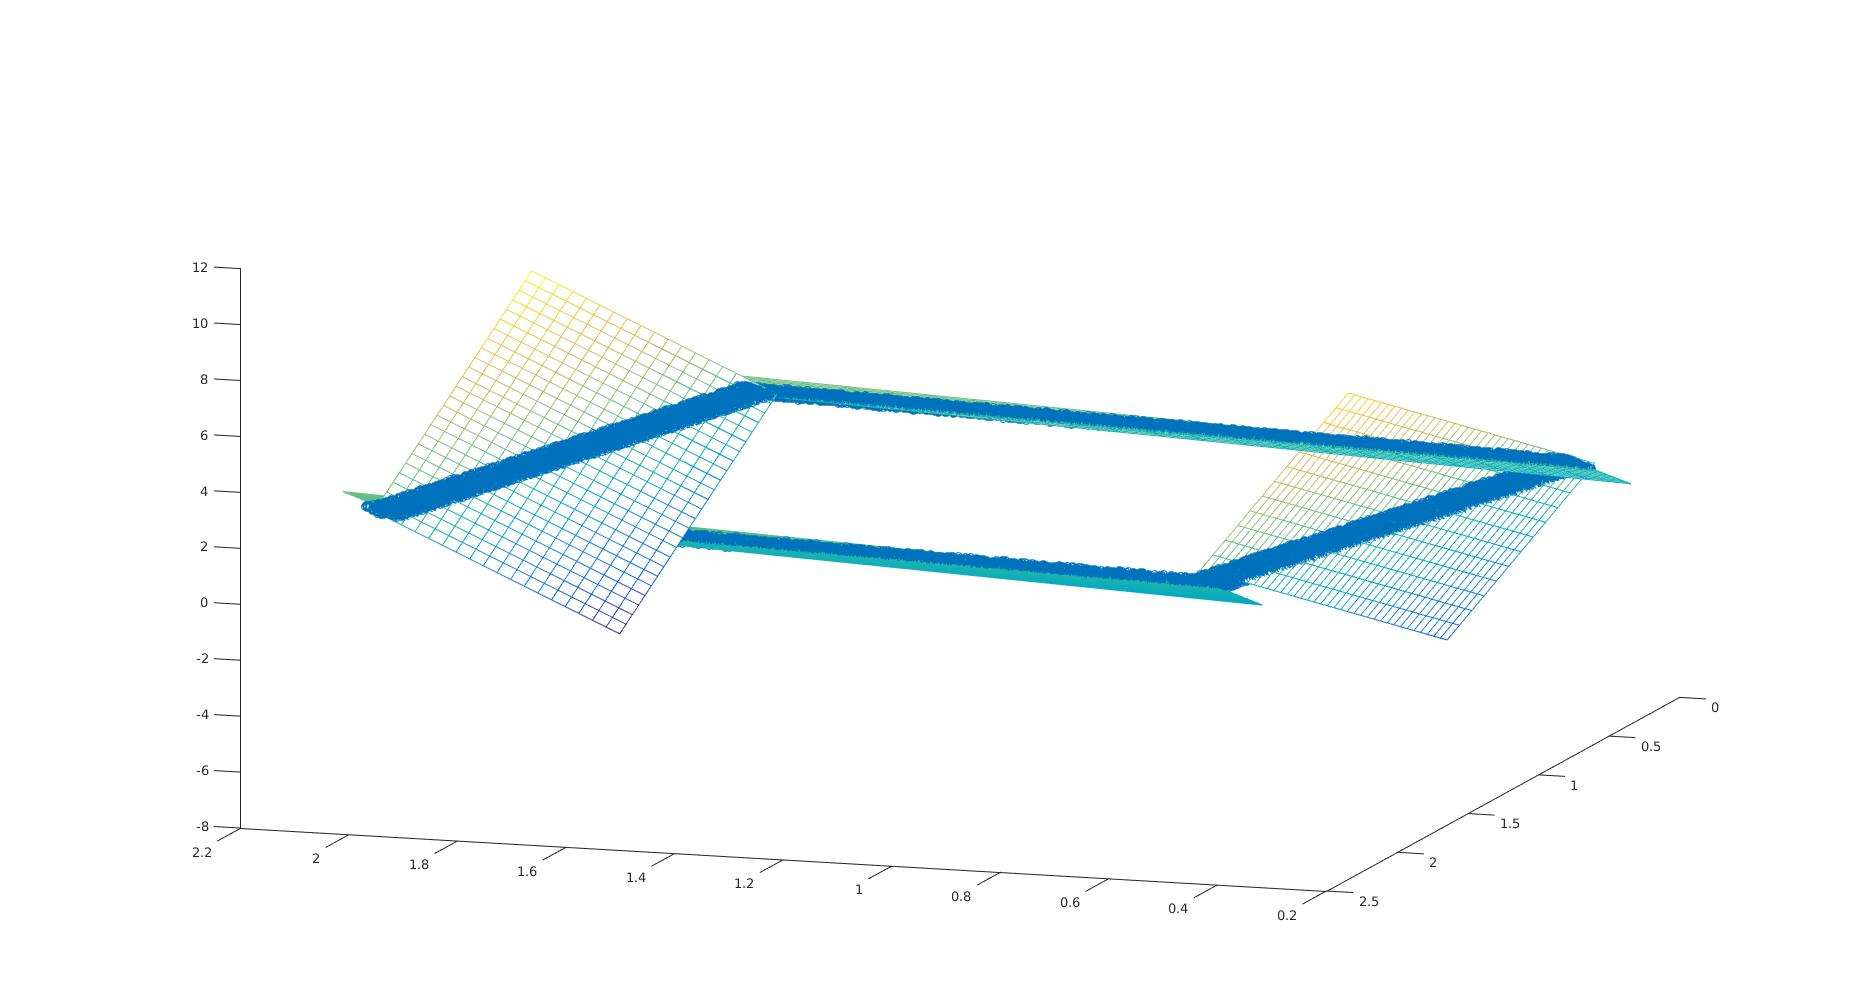
\includegraphics[width=5in]{figures/q4d.jpg}
\end{figure}
\begin{figure}[H]
\centering
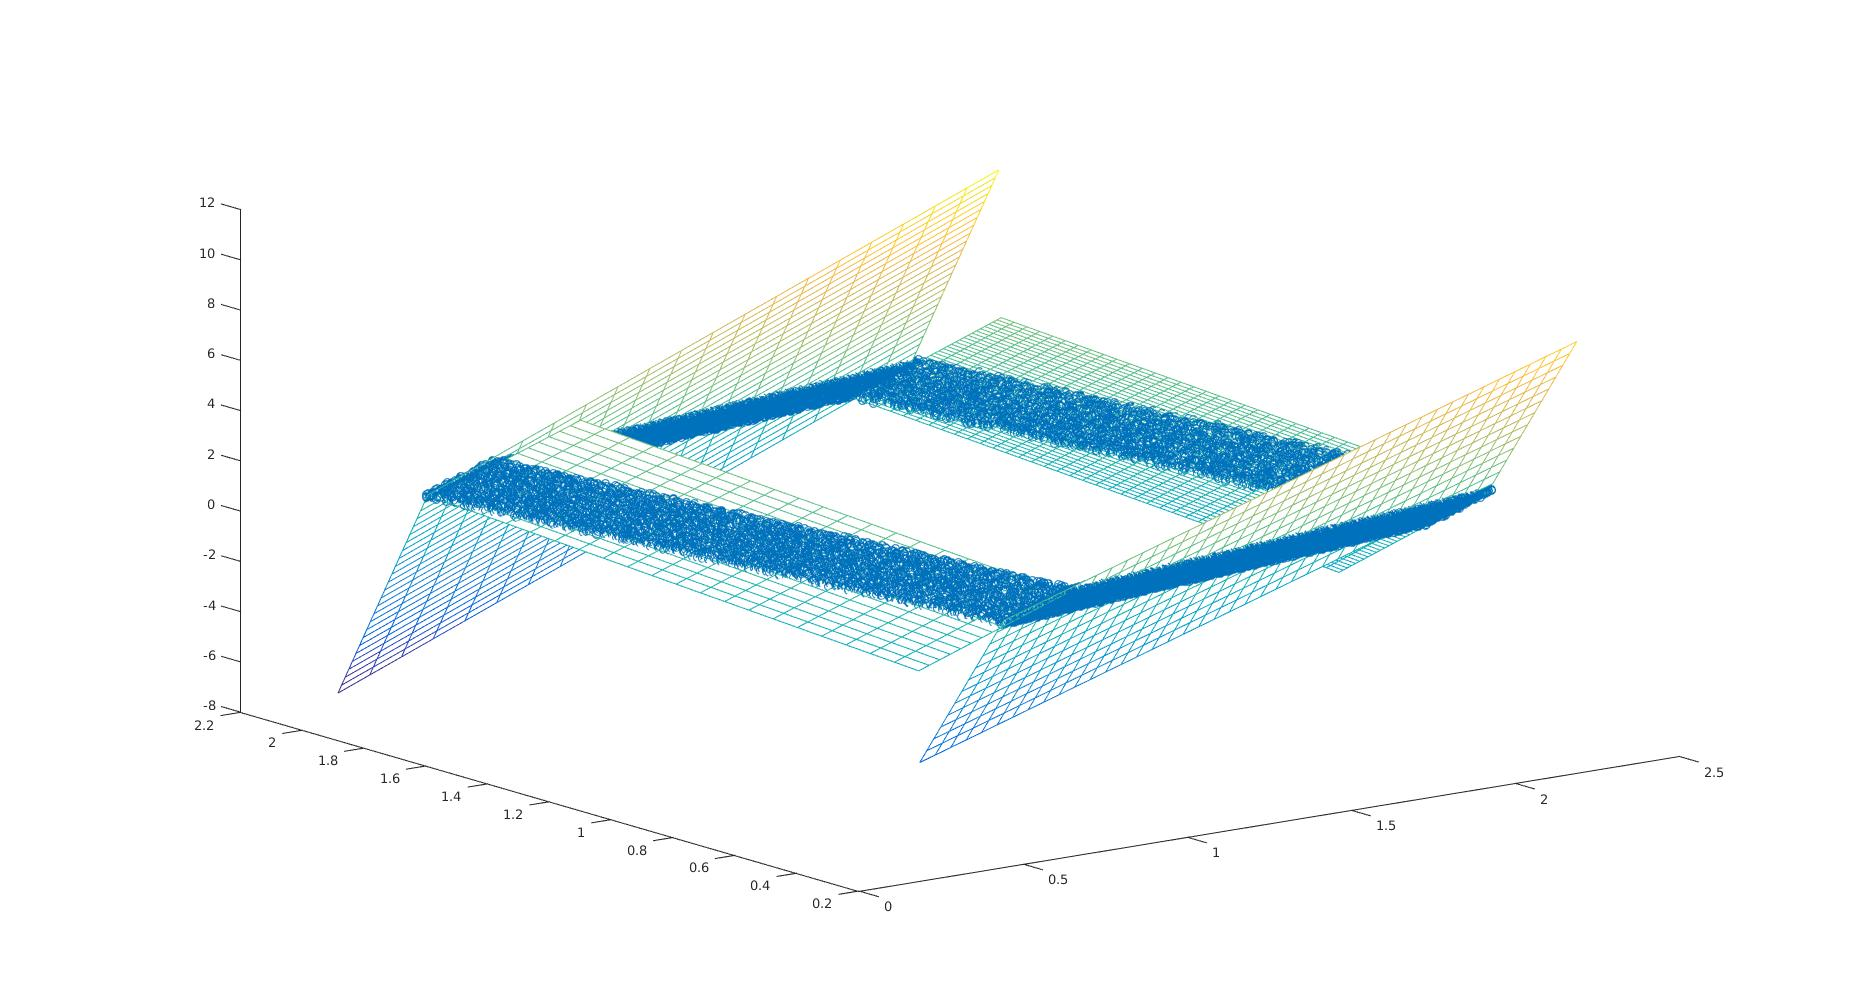
\includegraphics[width=5in]{figures/q4d-alt.jpg}
\end{figure}

\subsection*{4(e)}
When trying 4(e), our previous algorithm did not work because each plane no longer has the same amount of points. We improved our RANSAC to address this issue. The improved-improved RANSAC now first randomly pick one point from all possible points and instead of randomly picking other points, the algorithm will only pick points that are within a certain maximum range from the first point. The remaining algorithm is the same as \textbf{RANSAC\_imporved}. The implementation of the code can be found in \textbf{RANSAC\_3.m}.\\
Once we have created the need 4 planes, we created the following smoothness score. We notice that in the graph that an unsmooth surface while generates a plane, the distance between points and the plane are larger. Our smoothness score take advantage of this and calculate the average distance to the plane for each inlier points. The plane with the lowest score would be the best plane to travel. The implementation of the score function can be found in \textbf{smoothness.m}.\\
Following is the visualization of the planes, the red plane is the selected plane and the points that constructed the plan are colored blue. All the remaining points are those in yellow. The code to generate the graph can be found in \textbf{q4e.m}
\begin{figure}[H]
\centering
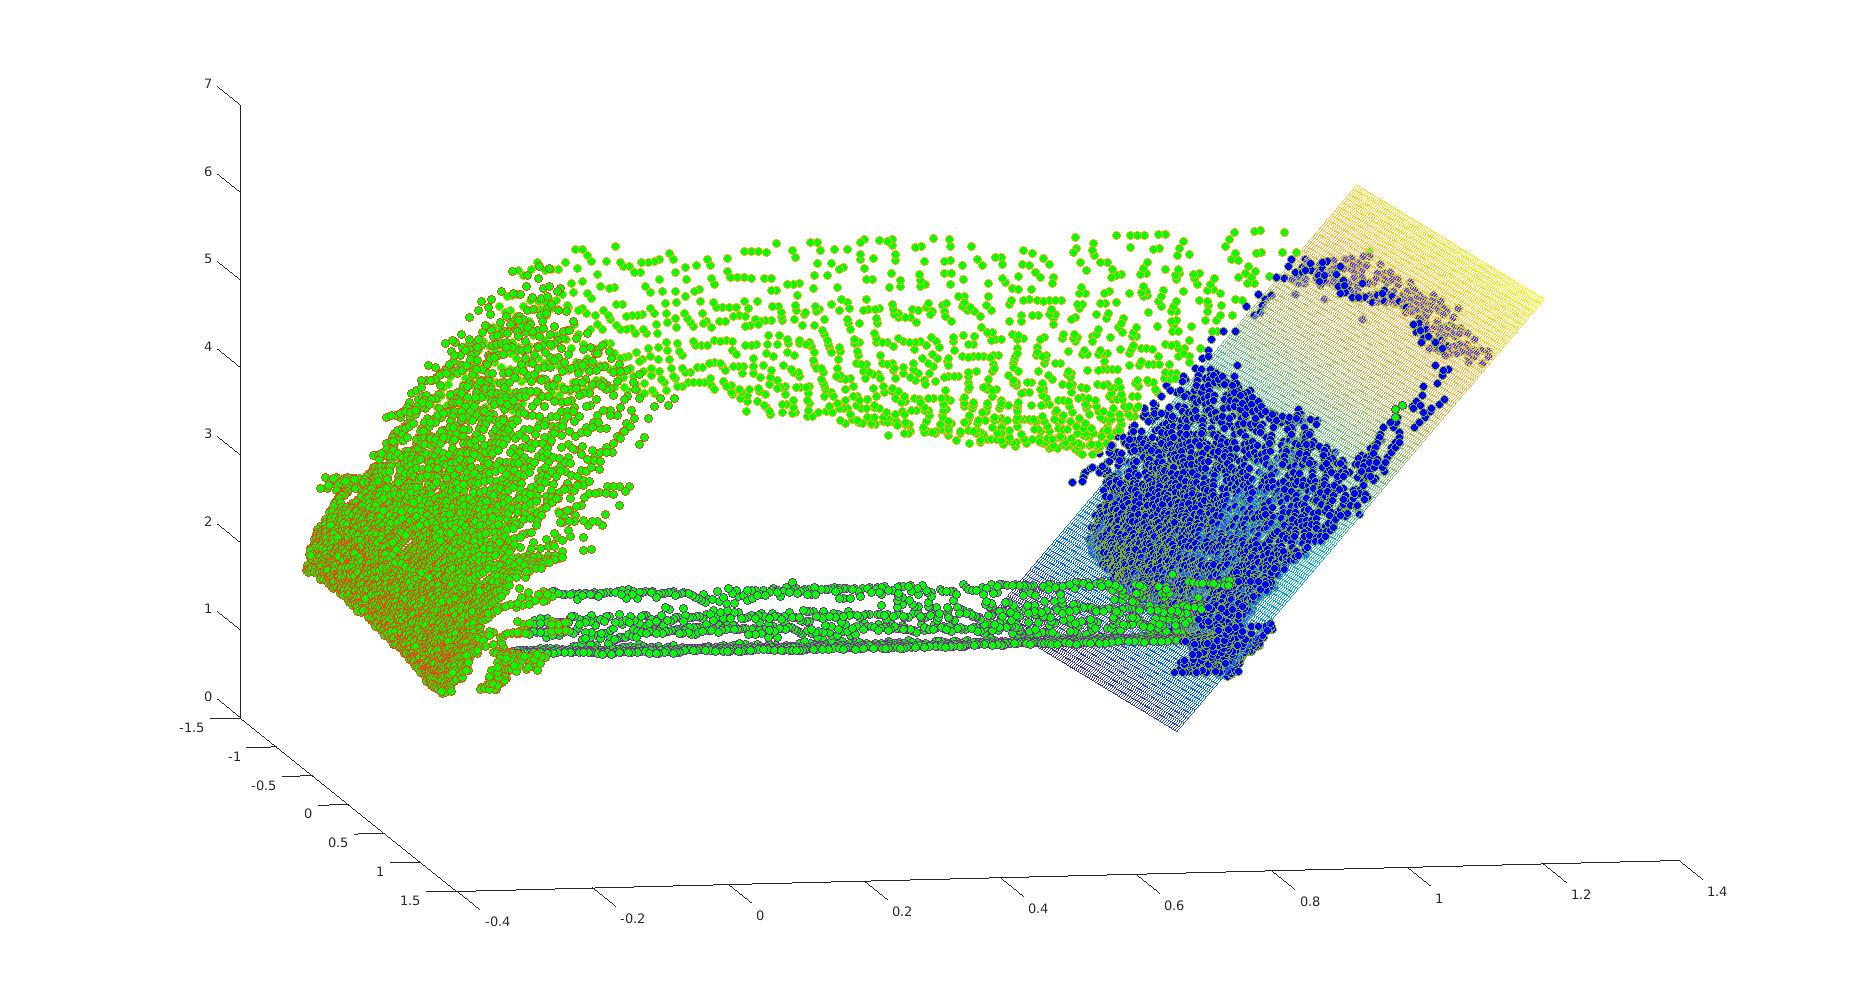
\includegraphics[width=5in]{figures/q4e.jpg}
\end{figure}
\begin{figure}[H]
\centering
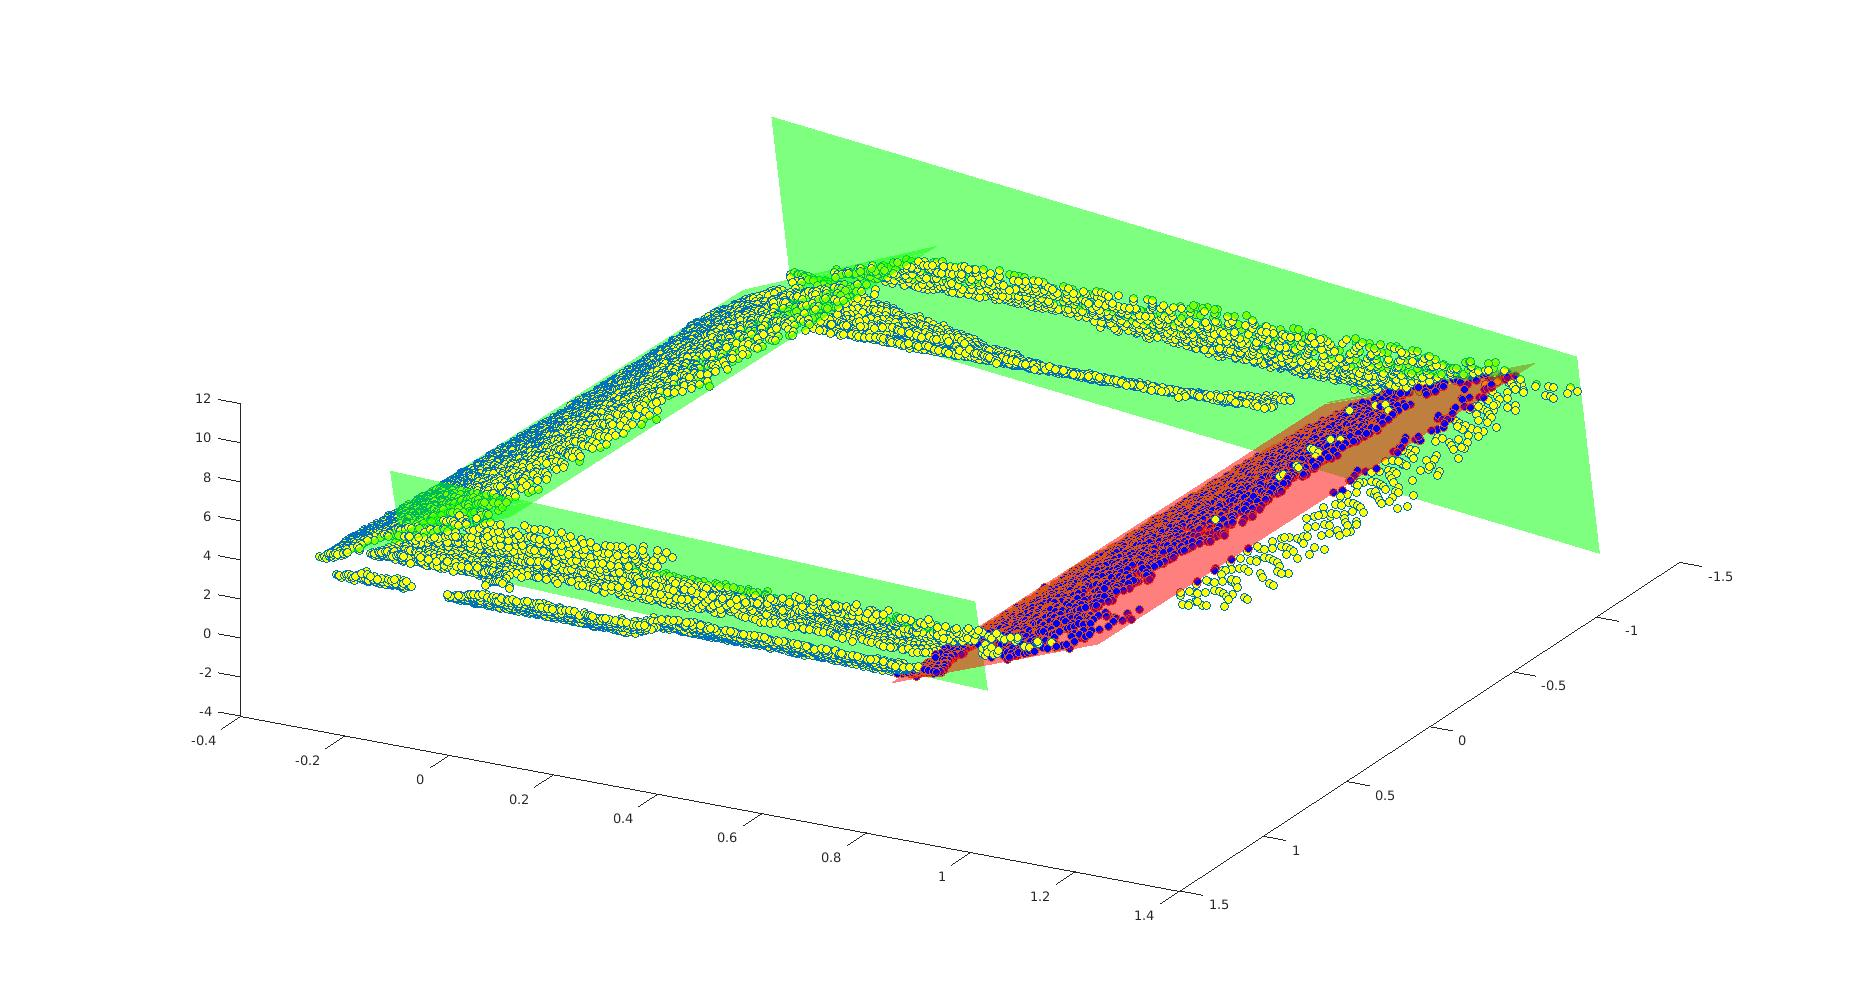
\includegraphics[width=5in]{figures/q4e-alt.jpg}
\end{figure}

\end{document}
